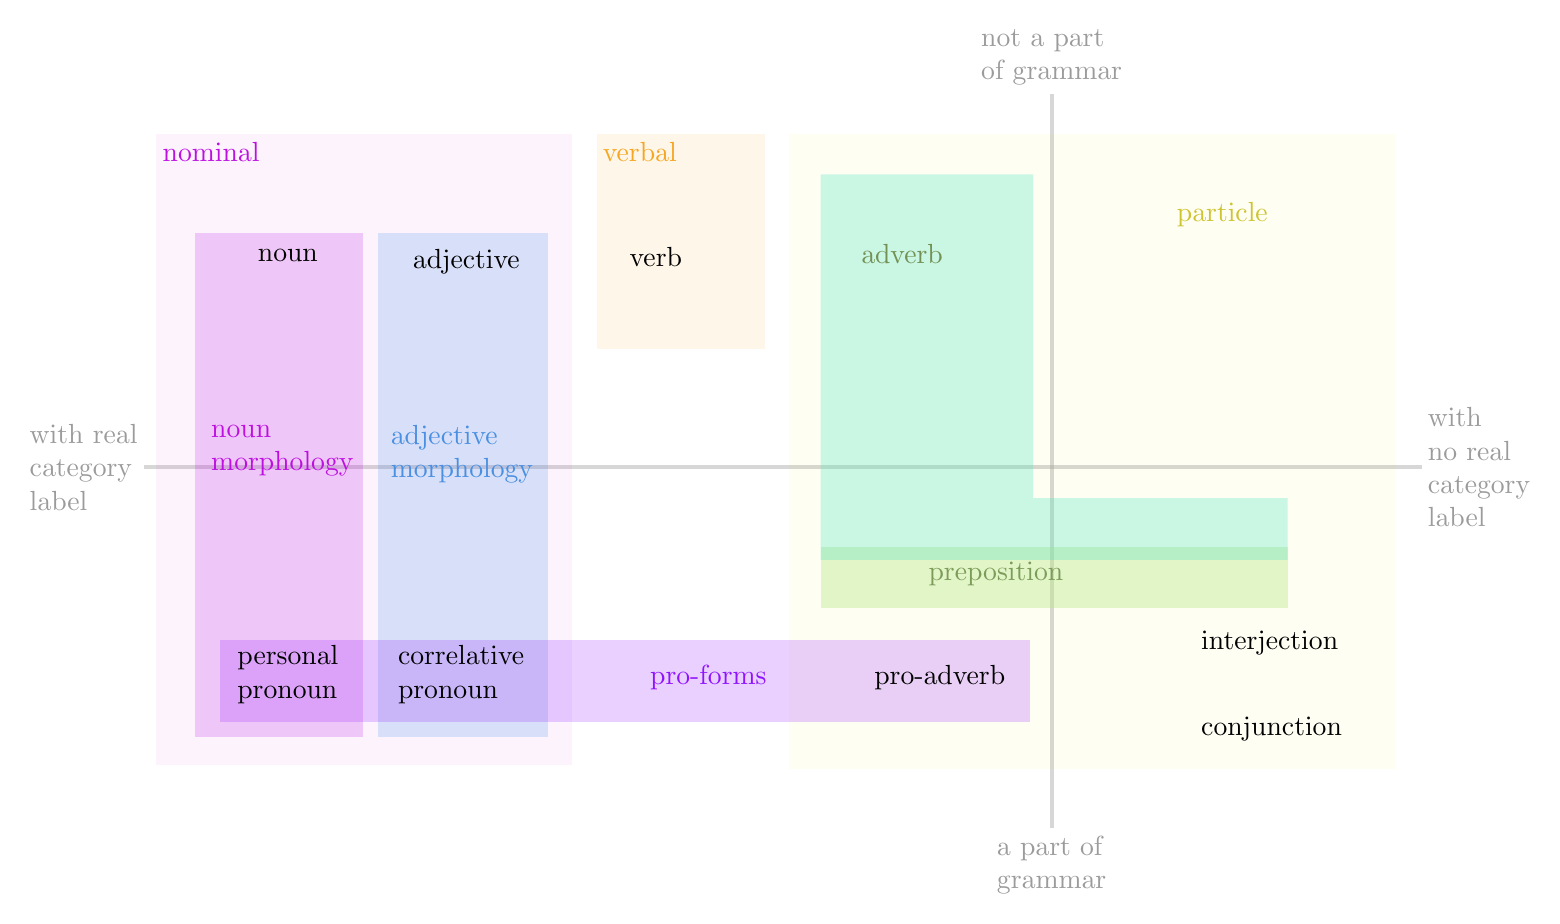
\begin{tikzpicture}[x=0.75pt,y=0.75pt,yscale=-0.9,xscale=0.9]
    %uncomment if require: \path (0,499); %set diagram left start at 0, and has height of 499
    
    %Straight Lines [id:da3400134236657377] 
    \draw [color={rgb, 255:red, 155; green, 155; blue, 155 }  ,draw opacity=0.4 ][line width=1.5]    (129.33,240) -- (813.33,240) ;
    %Straight Lines [id:da555192003881706] 
    \draw [color={rgb, 255:red, 155; green, 155; blue, 155 }  ,draw opacity=0.4 ][line width=1.5]    (615.33,433) -- (615.33,40) ;
    %Shape: Rectangle [id:dp5482669924039287] 
    \draw  [draw opacity=0][fill={rgb, 255:red, 189; green, 16; blue, 224 }  ,fill opacity=0.05 ][dash pattern={on 0.84pt off 2.51pt}] (136,61.6) -- (358.67,61.6) -- (358.67,399.6) -- (136,399.6) -- cycle ;
    %Shape: Rectangle [id:dp5557423002117736] 
    \draw  [draw opacity=0][fill={rgb, 255:red, 189; green, 16; blue, 224 }  ,fill opacity=0.2 ][dash pattern={on 0.84pt off 2.51pt}] (156.67,114.6) -- (246.67,114.6) -- (246.67,384.6) -- (156.67,384.6) -- cycle ;
    %Shape: Rectangle [id:dp40046124682601336] 
    \draw  [draw opacity=0][fill={rgb, 255:red, 74; green, 144; blue, 226 }  ,fill opacity=0.2 ][dash pattern={on 0.84pt off 2.51pt}] (254.67,114.6) -- (345.67,114.6) -- (345.67,384.6) -- (254.67,384.6) -- cycle ;
    %Shape: Rectangle [id:dp7865569568585418] 
    \draw  [draw opacity=0][fill={rgb, 255:red, 248; green, 231; blue, 28 }  ,fill opacity=0.05 ][dash pattern={on 0.84pt off 2.51pt}] (474.67,61.6) -- (799.67,61.6) -- (799.67,401.6) -- (474.67,401.6) -- cycle ;
    %Shape: Rectangle [id:dp5281825558720272] 
    \draw  [draw opacity=0][fill={rgb, 255:red, 184; green, 233; blue, 134 }  ,fill opacity=0.4 ][dash pattern={on 0.84pt off 2.51pt}] (491.67,282.6) -- (741.67,282.6) -- (741.67,315.6) -- (491.67,315.6) -- cycle ;
    %Shape: Rectangle [id:dp22517918869537135] 
    \draw  [draw opacity=0][fill={rgb, 255:red, 245; green, 166; blue, 35 }  ,fill opacity=0.1 ][dash pattern={on 0.84pt off 2.51pt}] (371.67,61.6) -- (461.67,61.6) -- (461.67,176.6) -- (371.67,176.6) -- cycle ;
    %Shape: Rectangle [id:dp5067363081477043] 
    \draw  [draw opacity=0][fill={rgb, 255:red, 144; green, 19; blue, 254 }  ,fill opacity=0.2 ][dash pattern={on 0.84pt off 2.51pt}] (170,332.6) -- (603.67,332.6) -- (603.67,376.6) -- (170,376.6) -- cycle ;
    %Shape: Path Data [id:dp48899049176074993] 
    \draw  [draw opacity=0][fill={rgb, 255:red, 80; green, 227; blue, 194 }  ,fill opacity=0.3 ][dash pattern={on 0.84pt off 2.51pt}] (741.67,256.6) -- (741.67,289.6) -- (491.67,289.6) -- (491.67,83.2) -- (605.4,83.2) -- (605.4,256.6) -- (741.67,256.6) -- cycle ;
    
    % Text Node
    \draw (189,122.09) node [anchor=north west][inner sep=0.75pt]   [align=left] {noun};
    % Text Node
    \draw (272,122.09) node [anchor=north west][inner sep=0.75pt]   [align=left] {adjective};
    % Text Node
    \draw (178,334.09) node [anchor=north west][inner sep=0.75pt]   [align=left] {personal \\pronoun};
    % Text Node
    \draw (264,334.09) node [anchor=north west][inner sep=0.75pt]   [align=left] {correlative \\pronoun};
    % Text Node
    \draw (388,121.09) node [anchor=north west][inner sep=0.75pt]   [align=left] {verb};
    % Text Node
    \draw (585.5,297.33) node  [color={rgb, 255:red, 124; green, 156; blue, 90 }  ,opacity=1 ] [align=left] {preposition};
    % Text Node
    \draw (694,372.09) node [anchor=north west][inner sep=0.75pt]   [align=left] {conjunction};
    % Text Node
    \draw (512,119.09) node [anchor=north west][inner sep=0.75pt]  [color={rgb, 255:red, 114; green, 145; blue, 83 }  ,opacity=1 ] [align=left] {adverb};
    % Text Node
    \draw (694,326.09) node [anchor=north west][inner sep=0.75pt]   [align=left] {interjection};
    % Text Node
    \draw (164,216.09) node [anchor=north west][inner sep=0.75pt]  [color={rgb, 255:red, 189; green, 16; blue, 224 }  ,opacity=1 ] [align=left] {noun \\morphology};
    % Text Node
    \draw (260.14,216.09) node [anchor=north west][inner sep=0.75pt]  [color={rgb, 255:red, 74; green, 144; blue, 226 }  ,opacity=1 ] [align=left] {adjective \\morphology};
    % Text Node
    \draw (127.33,240) node [anchor=east] [inner sep=0.75pt]  [color={rgb, 255:red, 155; green, 155; blue, 155 }  ,opacity=1 ] [align=left] {with real \\category \\label};
    % Text Node
    \draw (815.33,240) node [anchor=west] [inner sep=0.75pt]  [color={rgb, 255:red, 155; green, 155; blue, 155 }  ,opacity=1 ] [align=left] {with \\no real \\category \\label};
    % Text Node
    \draw (138,64.6) node [anchor=north west][inner sep=0.75pt]  [color={rgb, 255:red, 189; green, 16; blue, 224 }  ,opacity=1 ] [align=left] {nominal};
    % Text Node
    \draw (615.33,37) node [anchor=south] [inner sep=0.75pt]  [color={rgb, 255:red, 155; green, 155; blue, 155 }  ,opacity=1 ] [align=left] {not a part\\of grammar};
    % Text Node
    \draw (615.33,436) node [anchor=north] [inner sep=0.75pt]  [color={rgb, 255:red, 155; green, 155; blue, 155 }  ,opacity=1 ] [align=left] {a part of\\grammar};
    % Text Node
    \draw (519,344.59) node [anchor=north west][inner sep=0.75pt]   [align=left] {pro-adverb};
    % Text Node
    \draw (399,344.59) node [anchor=north west][inner sep=0.75pt]  [color={rgb, 255:red, 144; green, 19; blue, 254 }  ,opacity=1 ] [align=left] {pro-forms};
    % Text Node
    \draw (681,96.59) node [anchor=north west][inner sep=0.75pt]  [color={rgb, 255:red, 206; green, 195; blue, 49 }  ,opacity=1 ] [align=left] {particle};
    % Text Node
    \draw (373.67,64.6) node [anchor=north west][inner sep=0.75pt]  [color={rgb, 255:red, 245; green, 166; blue, 35 }  ,opacity=1 ] [align=left] {verbal};
    
    
    \end{tikzpicture}
    